\documentclass[10pt,journal,compsoc]{IEEEtran}

\usepackage[pdftex]{graphicx}    
\usepackage{cite}
\hyphenation{op-tical net-works semi-conduc-tor}


\begin{document}

\title{Localization with Customized Robots in Gazebo}

\author{Peng Xu}

\markboth{Localization project, Robotics Nanodegree Program, Udacity}%
{}
\IEEEtitleabstractindextext{%

\begin{abstract}
An indoor robot localization problem was investigated with two customized robots built in Gazebo. The robots were built from scratch and defined in urdf format. A differential controlled 2-wheel robot model was built from scratch and a skid steer 4-wheel robot was built based on the 2-wheel robot model. Both models were attached with Odometry, Lidar and camera sensors, which were reliable for localization applications. ROS and Rviz were used to control and visualize the localization and navigation experiments. The results indicated the localization in both cases were effective.
\end{abstract}

% Note that keywords are not normally used for peerreview papers.
\begin{IEEEkeywords}
4WD Robot, URDF, Gazebo, Kalman Filter, Monte Carlo Localization, Navigation Stack.
\end{IEEEkeywords}}


\maketitle
\IEEEdisplaynontitleabstractindextext
\IEEEpeerreviewmaketitle
\section{Introduction}
\label{sec:introduction}

\IEEEPARstart{T}{he} project is aiming for utilizing ROS packages to accurately localize a mobile robot inside a provided map in the Gazebo as shown in Fig. \ref{fig:intro} and RViz simulation environments.

%example for inserting image
\begin{figure}[thpb]
      \centering
      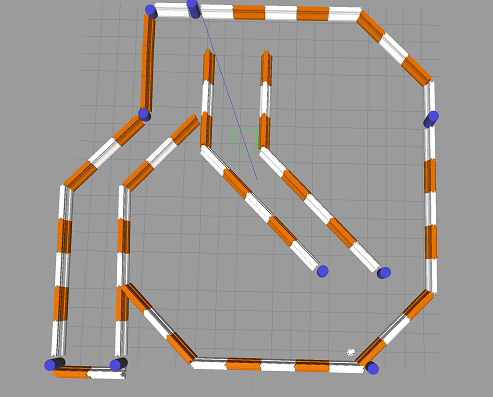
\includegraphics[width=\linewidth]{images/intro-image.png}
      \caption{Localization in a given map in Gazebo Simulator.}
      \label{fig:intro}
\end{figure}

Several aspects of robotics with a focus on ROS are got involved, including

\begin{itemize}
\item Building a mobile robot for simulated tasks.
\item Creating a ROS package that launches a custom robot model in a Gazebo world and utilizes packages like AMCL and the Navigation Stack.
\item Exploring, adding, and tuning specific parameters corresponding to each package to achieve the best possible localization results.
\end {itemize}

\subsection{Robot Simulation}
A robotics simulator is used to create application for a physical robot without depending on the actual machine, thus saving cost and time. In some case, these applications can be transferred onto the physical robot (or rebuilt) without modifications. Among those popular robotics simulators, such as V-REP \cite{vrep}, Gazebo \cite{gazebo} and ARGoS \cite{argos}, Gazebo stands out for several reasons. Firstly, it has abundant interfacing features with the widely used robotics framework, Robotic Operating System or ROS \cite{ros}. Secondly, it can utilize complex 3D meshes and physics engines, thought it lacks some features that V-REP has, such as mesh manipulation. Gazebo represents a middle ground between V-REP and ARGoS which makes the roboticist focused on the robotics problems instead of low level building work. Lastly and most importantly, the close-to-reality feature make it easy and fast to deploy the developed software on a real robot with subtle modifications.

As in this project, it is not a difficult work to build a two wheeled robot using differential controller and even a four wheeled robot using skid steer controller. The generally used sensors are also available to equip and stack on the robot using the according plugins, which will be described detailly in the later section.

\subsection{Robot Localization}
Nowadays, the field of mobile robotics is experiencing a quick evolution, and a variety of autonomous vehicles is available to solve different tasks. Nearly all of these applications require knowledge of the position of the robot; therefore it is necessary to perform a localization calculation. In localization, the position of the robot relative to a map of an environment is estimated and this calculation represents one of the most relevant problems in mobile robotics \cite{monte-carlo-localization-view}. Furthermore, these calculations are used in other modules of the robot control software that are in charge of deciding how the robot should act in the next movement. Reliable navigation in mobile robotics requires the computation of robust motion approximations. Solutions based on inertial measurement units or global positioning system (GPS) can provide position approximations and their corresponding uncertainties \cite{field-robot-localization}. However, this solution is impractical in indoor applications where GPS signals are not reliable. While outdoor localization in open areas has been largely solved with the advances in satellite-based GPS systems, indoor localization presents ongoing challenges due to the large range of variables that require different techniques \cite{indoor-localization-solution}. As it is not possible to have a calculation using GPS, the use of other types of sensors, such as Lidar (Light Detection and Ranging), camera and IMU (inertial measurement unit),is necessary to collect information from the environment. 

From the view point of Probabilistic Robotics, the current location of the robot can be estimated by the use of the information of all previous robot locations \cite{probabilistic-robotics}. Consider a robot with an internal map of its environment. When the robot moves around, it needs to know where it is within this map or determine its location and rotation (more generally, the pose) by using its sensor observations, which is known as robot localization with known maps. In this process, a lot of noise coming from the sensors themselves and the mathematical models have to be taken into account. Probabilistic state estimation methods such as Kalman Filters \cite{kalman-filter-intro} and Monte Carlo Localization (or Particle Filters) \cite{mcl-intro} methods can be used to capture the robot state (or pose here) as accurate as possible.

\section{Background}

Indoor robot localization, due to the lack of global positioning information, requires feature based estimation. Several methods were investigated and finally Adaptive Monte Carlo Localization (AMCL) method stands out due to its convenience and good performance. 

\subsection{Kalman Filters}

The Kalman filter based techniques are based on the assumption that uncertainty in the robot’s position can be represented by a unimodal Gaussian distribution. Kalman filter based techniques have proven to be robust and accurate for keeping track of the robot’s position. However, this approach cannot deal with multi-modal densities typical in global localization. The other limitation is that the initial posture must be known with Gaussian uncertainty at most. 

\subsection{Monte Carlo Localization}

Monte Carlo Localization uses randomized samples to represent a robot’s belief about its location in an environment and is notable for its accuracy, efficiency, and ease of use compared to previous approaches. MCL was first presented in 1999 \cite{mcl-intro} and was the first application of sample-based estimation in robotics, where it is now used across a wide range of application.

The global localization problem particularly is difficult to solve because it involves a robot which is not told its initial position; the position tracking problem is the most-studied problem that a robot knows its initial position and only has to accommodate small errors as it moves.

By using a sampling-based representation, MCL has several key advantages over earlier work in the field \cite{acl-advantages}:

\begin{itemize}
    \item In contrast to existing Kalman filtering based techniques, it is able to represent multi-modal distributions and thus can globally localize a robot.
    \item It drastically reduces the amount of memory required compared to grid-based Markov localization and can integrate measurements at a considerably higher frequency. The online algorithm lends itself nicely to an any time implementation.
    \item It is more accurate than Markov localization with a fixed cell size, as the state represented in the samples is not discretized.
    \item It is much easier to implement.
\end{itemize}


\subsection{Adaptive Monte Carlo Localization}

A key problem with traditional MCL is maintaining the random distribution of particles throughout the state space, which goes out of hand if the problem is high dimensional. Due to these reasons it is much better to use an adaptive particle filter which converges much faster and is computationally much more efficient than a basic particle filter.

The key idea is to bound the error introduced by the sample-based representation of the particle filter. To derive this bound, it is assumed that the true posterior is given by a discrete, piece-wise constant distribution such as a discrete density tree or a multidimensional histogram. For such a representation we can determine the number of samples so that the distance between the maximum likelihood estimate (MLE) based on the samples and the true posterior does not exceed a pre-specified threshold. As is finally derived, the number of particles needed is proportional to the inverse of this threshold \cite{adaptive-pf}.

\section{Simulations}

The robot models were built from scratch in Gazebo which at least offered one advantage over a third -party model, the full access to the model features and parameters. Accordingly, the parameters would be tuned for each model to give an intuitive understanding.

A two wheeled robot using differential controller, called "udacity bot", was firstly built following a general guideline which would be used as a benchmark model. The use of the differential controller made it mathematically simple to compute and easy to operate, making it a good starting point.

Based on the two wheeled robot, a four wheeled robot called "rover bot", was then built by adding two wheels in parallel. The modified robot was using the skid steer controller.

\subsection{Achievements}

Both the benchmark model and the modified model presented the ability to localize themselves using AMCL and delivered themselves to the goal position with the desired orientation successfully. Their performance would be described in the next sub-sections.

% Robot Models
\subsection{Benchmark Model}

\subsubsection{Model design}

The benchmark robot, "udacity bot", is simply a cuboidal (or box) as the chassis or the body and two wheels positioned on the two sides. Two caster wheels are attached under the chassis as a whole for the balance. The sizes of the chassis and the wheels are shown in Table \ref{tab:udacity-bot-size}. The Hokuyo Lidar is placed on the front top of the chassis and the camera is put in the front of the chassis. The robot also is colored with different colors indicating different materials. The final rendered model is as shown in Fig. \ref{fig:udacity-bot}. In Gazebo, one or more so-called "urdf" format files are storing these parameters. The "urdf" files are one kind of xml format files which easily describe the hirachical architecture of the robot components from the base link as the parent link to child links and even the child links of the child links.

\begin{table}[h]
    \caption{The size information of the benchmark model "udacity bot"}
    \label{tab:udacity-bot-size}
    \centering
    \begin{tabular}{c|c}
    \hline
    Component & Size \\
    \hline
    Chassis & Length:0.4 m, Width:0.2 m, Height: 0.1 m \\
    \hline
    Caster Wheel & Radius: 0.0499 m \\
    \hline
    Wheel & Radius: 0.1 m, Length: 0.05 m\\
    \hline
    \end{tabular}
\end{table}

\begin{figure}[thpb]
    \centering
    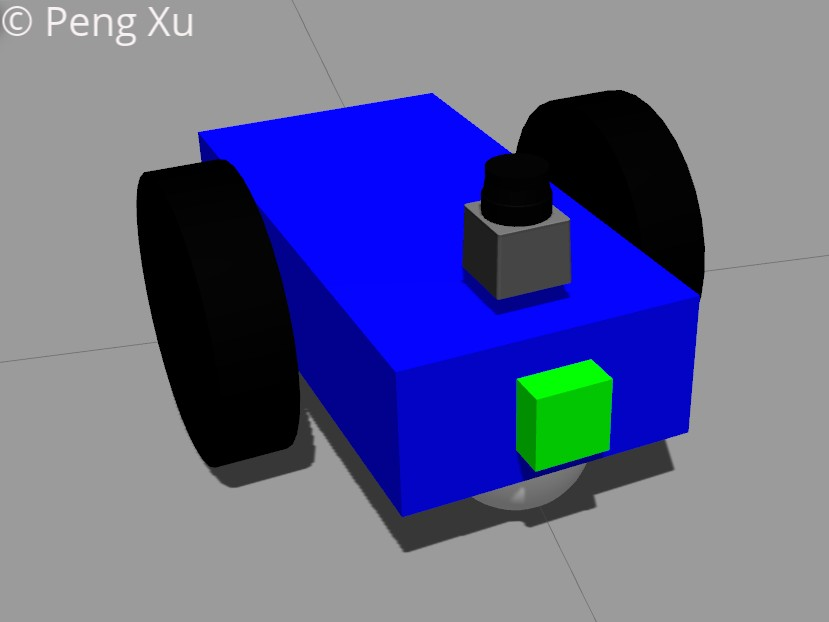
\includegraphics[width=\linewidth]{images/udacity-bot.png}
    \caption{Benchmark model: Udacity Bot. A two wheeled robot using differential controller.}
    \label{fig:udacity-bot}
\end{figure}

A static robot model is built by adding the links as above and the joints which attach them together and define their relative motion like rotation of wheels. But how to make it drivable? A controller is necessary to be defined then. There are some predefined motion controllers that can be referenced as a plugin in the urdf files so one can use rostopic to command it just like a real robot. In here, a "differential controller" as a plugin is introduced.

\subsubsection{Packages Used}

The packages used in the project could be devided into three parts,

\begin{itemize}
    \item Loading the models.
    \item Running the localization software.
    \item Sending the goal and run the navigation.
\end{itemize}

The robot model will be relying on the two packages, "joint\_state\_publisher" and "robot\_state\_publisher" to communicate with the ROS controller software and indicate its state.

A package called "gazebo\_ros" will be responsible for loading all the models, include the world or the track model and the robot model into Gazebo.

Till now, the robot is good to be loaded and driven by ROS commands.

The "amcl" package will apply AMCL algorithm and publish the odometry in topic "\slash odom" based on the Lidar scan information in topic "\slash{udacity\_bot}\slash{laser}\slash{scan}" and the given 2D map in topic "\slash map".

The "move\_base" package from the Navigation Stack software will generate motion plans for the robot and lead it to the goal position and orientation.

\subsubsection{Parameters}

There are some parameters in the AMCL node and move\_base parameters in the configuration files which are essential for the location and navigation to work properly.

In both amcl.launch and costmap\_common\_params.yaml, the parameter "transform\_tolerance" is the time with which to post-date the transform that is published, to indicate that this transform is valid into the future. It needs to be tuned for successfully and stably generating the \slash{odom} message. I set it as 0.3 after the trials.

Both "update\_frequency" and "publish\_frequency" in global\_costmap\_params.yaml and local\_costmap\_params.yaml were decreased a little for quicker response since the computing power is good enough. 

In amcl.launch file, the initial pose of the robot should be set as 0 as an origin point. The parameters "min\_particles" and "max\_particles" defines the range of particle number used to estimate. The number needs to be set not too small for the accuracy and not too big for the computation effiency. I finally pick 100 and 500 respectively for them.

\subsection{Personal Model}

The benchmark model was expected to be modified in any aspects such as component shapes, the sensor displacement, materials, etc. 

\subsubsection{Model design}

\begin{figure}[thpb]
    \centering
    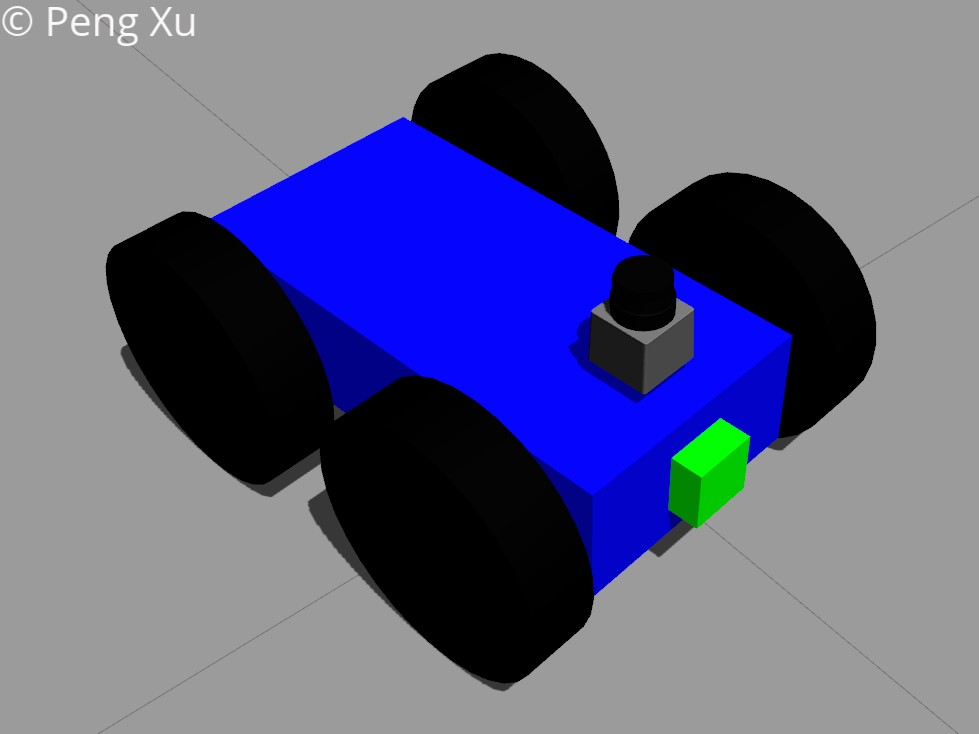
\includegraphics[width=\linewidth]{images/rover-bot.png}
    \caption{Personal model: Rover Bot. A four wheeled robot using skid steer controller.}
    \label{fig:rover-bot}
\end{figure}

As shown in Fig. \ref{fig:rover-bot}, the main modification from the benchmark model is to add two more wheels positioned in parallel with the original two. In the end, two of them were shifted to the front and the other were moved to the back. The distance of the two pairs is 0.25 meters. The radius of the wheels was increased 25\% to 0.125 for better turning performance. As the robot model now is relying on the four wheels, the controller according needs to be changed from "differential" to "skid steer". A new Gazebo plugin will replace the differential controller plugin. The modified model is called "Rover Bot".

One of the key reasons for this modification is to make this simulated robot better serve the real world counterpart, as shown in Fig. \ref{fig:roverpi-18650}. The robot is made with a four wheeled chassis and a Raspberry Pi 3 b+ board installed ROS Kinetic. The detailed description will be presented in later sections or future work.

\begin{figure}[thpb]
    \centering
    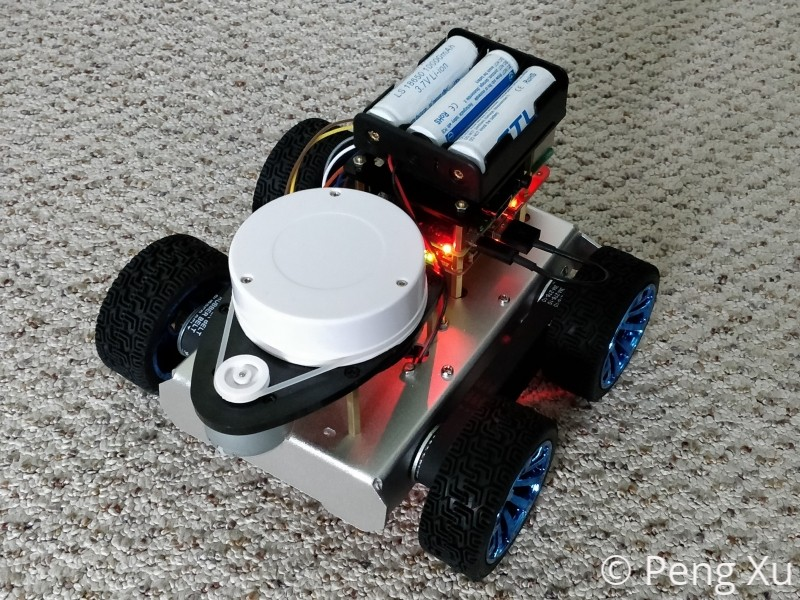
\includegraphics[width=\linewidth]{images/roverpi-18650.jpg}
    \caption{RoverPi Bot using Raspberry Pi and ROS Kinetic.}
    \label{fig:roverpi-18650}
\end{figure}

\subsubsection{Packages Used}

The packages used for Rover Bot inherit from those for Udacity Bot and are almost the same.

\subsubsection{Parameters}

There parameters are kept the same unless a big feature changed.

\section{Results}

The localization results look reasonable for the both robot models. The performance will be presented from the following aspects:

\begin{itemize}
    \item The duration for the particle filters to converge.
    \item The elapsed time it takes for the robot to reach the goal.
    \item How it follows the path to the goal.
    \item Does it have unexpected behavior in the process?
\end{itemize}

\subsection{Localization Results}

Both the benchmark and the modified robots performed similarly since they have similar mass, size and actuators.

It took around 3 seconds to converge for the particle filters and about 30 to 40 seconds to reach the goal. The moving path was quite smooth except for a pause at the turning point for both robots. Especially, when the either robot reach the goal position, it took about 1 second to rotate to the desired orientation.

\begin{figure}[thpb]
    \centering
    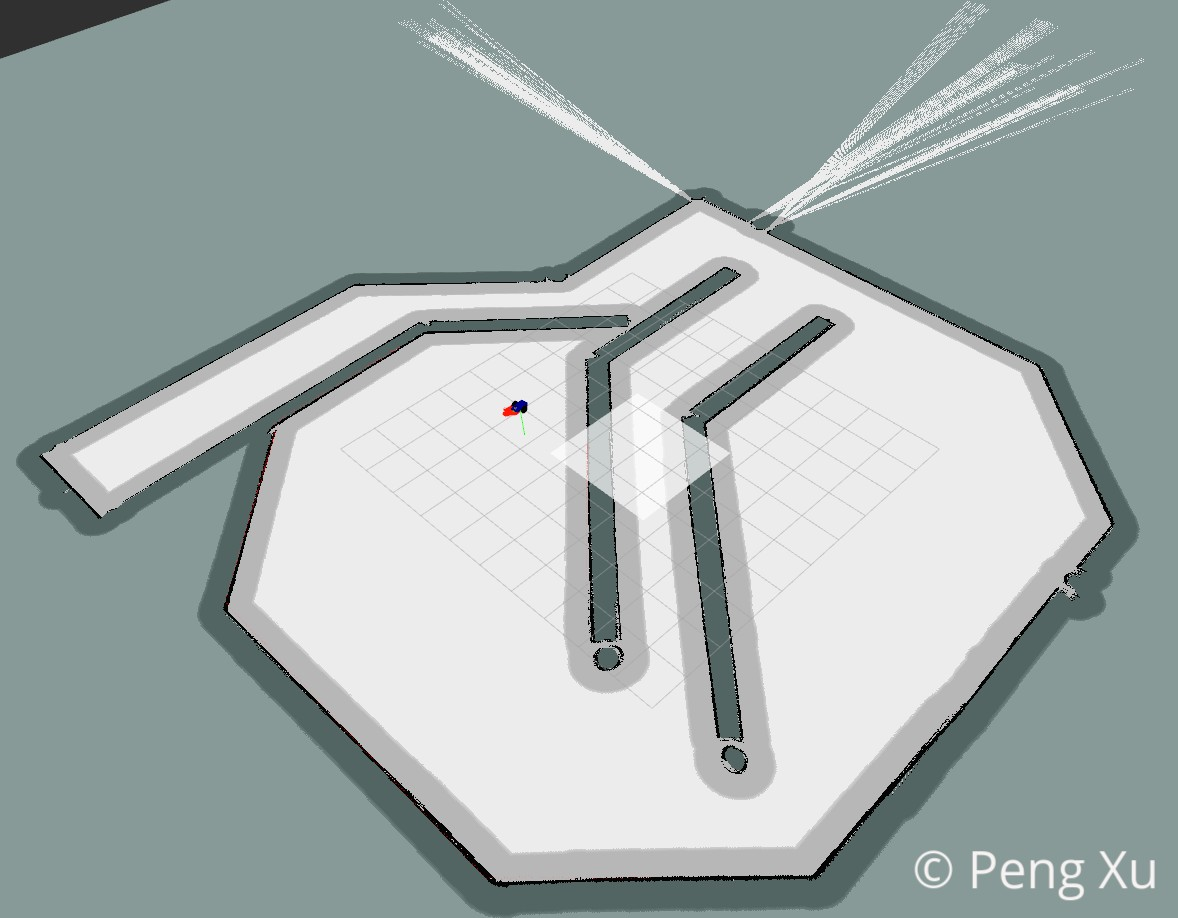
\includegraphics[width=\linewidth]{images/udacity-bot-rviz-final.png}
    \caption{Benchmark model localization result.}
    \label{fig:udacity-bot-finish}
\end{figure}

\begin{figure}[thpb]
    \centering
    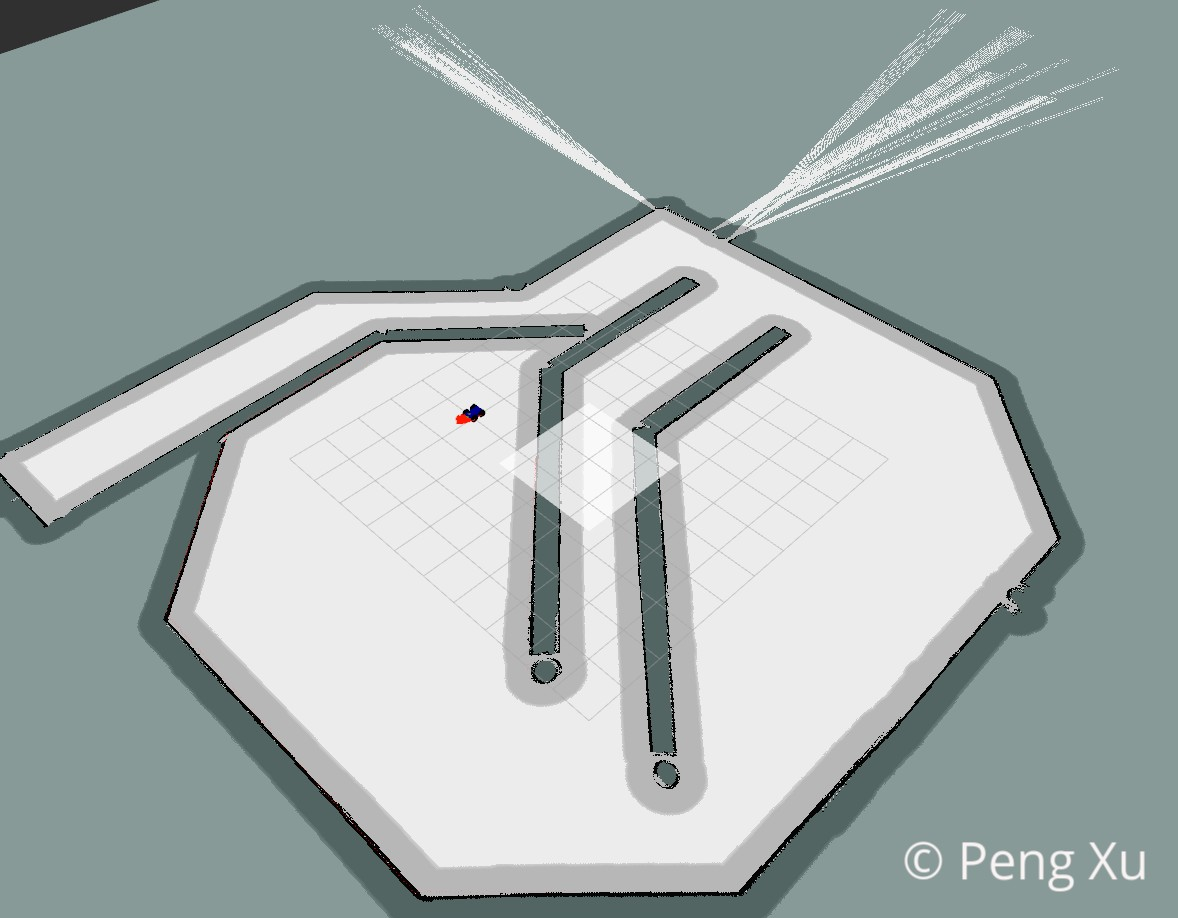
\includegraphics[width=\linewidth]{images//rover-bot-rviz-final.png}
    \caption{Personal model localization result.}
    \label{fig:rover-bot-finish}
\end{figure}

\subsection{Technical Comparison} % only facts

The skid steer controller is nothing more than the four wheeled version of the differential controller. Thus, the modified robot model inherited the most advantages from the benchmark one, such as mechanism simplicity. In addition, multiple drive wheels on each side gives greatly increased traction, especially on rough terrain (even greater for tracked vehicles). On the other hand, what has been sacrificed in this process is the accurate control and measurement of the motion because skidding causes wheels to lose contact with the ground which means odometry sensors cannot accurately track the position of the robot. This issue can be addressed by the use of other kinds of range detect sensors like inertia measurement unit (IMU) and Lidar. Since Lidar is more reliable to give a localization measurement here, this lose can be igored.

\section{Discussion}

The modification in this project was conservative and didn't result a strong challenge of the performance. This may be good enough to be familiar with the pipeline of building a robot from scratch but remains deep investigation work in the next step.

The particles have quickly converged in the experiments which demonstrate that AMCL is effective and robust.

The both robots performed almost equally in localization tasks since they share most features in shapes and senser placement. The adopted method, AMCL, is perfect to address the "Kidnapped Robot" problem. Differing from Kalman Filter based methods, MCL or AMCL is a global localization method which doesn't relying on the initial or the previous robot poses but the particles to estimate the new robot pose. In this way, even if the robot is kidnapped it still have chance to converge after a few of steps. The indoor robot will be a promising scenario for this method to be more widely used. As for the industry domain, the warehouse robot could also need MCL or AMCL to be used.

\section{Conclusion}

The project successfully demonstrated the effectiveness of AMCL algorithm in Gazebo simulator by the use of two customized robots. The communication and motion control is close to reality making it simple to be transferred to a real world robot.

For Future Work, address areas of work that you may not have addressed in your report as possible next steps. This could be due to time constraints, lack of currently developed methods / technology, and areas of application outside of your current implementation. Again, avoid the use of the first-person.

\subsection{Modifications for Improvement}

THe basic dimension of the robot model, Rover Bot, is satisfying but still fine to have more trials, like changing the cubic to a circle which makes like a mopping robot for home service. More sensors such as more cameras and an IMU could be introduced to have a broader view of the environment which may bring in a new problem, sensor fusion, which is another interesting topic in robotics and autonomous systems.

\subsection{Hardware Deployment}

As shown in Fig. \ref{fig:roverpi-18650}, the real world robot RoverPi Bot, would be a good platform to experiment the same pipeline on the simulated one. The RoverPi Bot has been prepared for basic motion control and sensor connection. The next step would be to use a ROS node and the "cmd\_vel" topic to drive the robot.

\bibliography{bib}
\bibliographystyle{ieeetr}

\end{document}